\documentclass[conference]{IEEEtran}
\usepackage[pdftex]{graphicx}
%\usepackage{epstopdf}
\graphicspath{{./png/}{./eps/}}
\DeclareGraphicsExtensions{.pdf,.png}
\usepackage[caption=false,font=footnotesize]{subfig}
\hyphenation{op-tical net-works semi-conduc-tor}
\begin{document}
\title{The design and implementation of standards-based Grid single sign-on using federated identity}

\author{\IEEEauthorblockN{Weizhong Qiang, Aleksandr Konstantinov}
\IEEEauthorblockA{Department of Physics, University of Oslo}
}

\maketitle


\begin{abstract}
Security infrastructure is one of the most challenging tasks in the developement, integration and
deployment of Grid middlewares. Even though the Grid community addresses the security issue 
through public key infrastructures (PKI) to support mutual authentication using X.509 certificates,
maintaining the X.509 credential is not that easy for non-IT specialists, and is proved to be an 
obstacle for the more widely deployment of Grid technology. Considering the identity federation 
technology is a emergingly widely used technology which can facilitate cross-domain single sign-on,
without requiring the users to maintain the X.509 credentials rather than their own institutional
accounts, we believe utilizing identity federation for Grid middlwares is a promising direction 
for Grid technology to be more widely used.
This paper describes a single sign-on infrastructure developed as part of the NorduGrid/ARC grid 
middleware. It adopts the identity federation standard (SAML), as well as Web Service standand. 
It focus on single sign-on solution on the middleware level for users to access Grids by only 
using their frequently used accounts, without being bothered to maintain X.509 credentials. 
Unlike other research which utilize identity federation on the Grid portal level, solution on
the middleware level can provide more flexibility.
Also, the performance of single sign-on solution is measured. We identify the performance limitation 
of security-related services inside this solution, and analyze the ways to avoid the limitation.
To our knowledge, the work described in this paper is the first evaluated implementation that utilizes 
identity federation for Grid usage on the middlware level.
\end{abstract}

%-------------------------------------------------------------------------
\section{Introduction}
\label{sec:intro}
Grid infrastructures facilitate the interoperability between wide-scale, cross-domain heterogeneous 
resources, as well as the accessibility provided to users. In terms of security issue, the Grid security 
infrastruture should provide accessibility as much as possible without loosing the security benifits.

The current Grid community uses Grid Security Infrastructure (GSI)~\cite{IFoster98} as the de facto 
standard for authentication and transport level security, which builds on the Public Key Infrastructure
(PKI) to support authentication using X.509 certificate. Mutual authentication is required 
by GSI based Grid deployment. Mutual authentication means that Grid users have to possess X.509 
credentials. To obtain a X.509 credential, a user needs to contact the Registration Authority (RA)
which will check the user's information and approve his certificate request; afterwards,
the Certificate Authority (CA) can issue the certificate according to the approval from 
the RA. The whole process is arduous and may take some time.
Meanwhile, to maintain a X.509 certificate is also not so easy for the non-IT community to deal 
with, since users have to periodically create proxy certificates by using Grid-specific command line 
utilities, such as grid-proxy-init or voms-proxy-init. Also maintaing the CAs or RAs is not a  
easy task, especially when the community of Grid users is getting much wider.

On the other hand, users normally could already have had some frequently-used campus or institutional 
accounts/credentials such as username/password. We believe that enabling Grid users to use their institutional 
credentials rather than the X.509 certificate to access Grids is a promising way 
to make the Grids more easily accessible, as well as to extend the user community of Grids
to a much larger scale.

To enable users to utilize the institutional credentials to access Grid, some issues needs to be 
addressed. Firstly, the Grid middleware needs to be improved to support the authentication based on
institutional credentials instead of X.509 certificates; Secondly, in order to interoperate with
those Grid infrastructures which require X.509 certificate based mutual authentication, an approach
should be provided for obtaining X.509 certificate based on the institutional credentials; Thirdly,
the single sign-on characteristic should be provided so that users can authenticate once and then transverse 
from Grid resources to Grid resources without being prompted to authenticate again at each of the resources.

The approach in the new version of ARC grid middleware is to utilize the identity federation 
standards, specifically, the Security Assertion Markup Language (SAML) specification, and Web 
Service standards, to facilitate the Grid single sign-on.

The rest of this paper is organized as follows: Section \ref{sec:arcmiddleware} presents the 
ARC Grid middleware, especially the architecture of the new version of ARC. Section 
\ref{sec:intergrationSAML2SSO} describes the solution of using federated identity for 
Grid authentication by using SAML2SSO profile; Setion \ref{sec:fedidtoX509} describes
how to obtain a X.509 credential based on federated identity, and how to use it for 
accessing multiple Grid resources; Section \ref{sec:perfeval} is performance evaluation;
Section \ref{sec:relatedwork} describes the related work; Section \ref{sec:conclusion} 
contains conclusions and future work outlook.

%-------------------------------------------------------------------------
\section{ARC Grid middleware}
\label{sec:arcmiddleware}

ARC (Advanced Resource Connector) is an open source Grid middleware solution released 
under Apache license. ARC middleware aims at developing self-organized, 
fault-tolerant, non-intrusive, easy-manageable Grid middleware~\cite{MEllert07}. 
The current production version of ARC provides Grid services for job submission and 
management, resource characterization, resource aggregation and discovery, basic data 
management, integration of Grid security solution, and so on. This release has been 
deployed and used in production environment, and is one of the widely deployed Grid 
middlewares in Europe.

The development version of ARC components is developed by the KnowARC project~\cite{KnowARClink}, 
based on the functionality of the current production ARC middleware. It aims at 
implementing a Web Service oriented Grid middleware which will provide higher levels of 
resource and user abstraction through well-defined Web Service interface~\cite{KnowARCDesignlink} 
in order to provide interoperability with other Web Service oriented Grid middlewares, as well as 
other Web Service compatible applications.

As the key part of the implementation of new ARC middleware, there is a lightweight Web 
Service container called Hosting Environment Daemon (HED) which provides hosting environment 
for various services at application level, as well as a number of modules to support flexible, 
interoperable, and efficient communication mechanism for building SOAP based Web Services. 
The design of the HED is built around the idea of flexibility and modularity,
such that the application service developers can simply concentrate on the application 
level Web Service implementation by only using the core minimum amount of components. It 
also simplifies work on the middleware level, e.g. making possible to implement another 
communication protocol or authentication mechanism. A system administrator can easily 
configure and deploy the middleware and application for different kinds of requirements 
without having to know much about the implementation. 

The architecture of the HED is illustrated in Figure \ref{fig:HED}. In general, there 
are few components called Message Chain Component (MCC) which are in charge of implementing 
different protocol levels. For instance, as shown in the example message flow, the HTTP MCC 
will process stream from the TLS MCC to parse the HTTP message and pass its body to the SOAP 
MCC, and also process the SOAP response from the SOAP MCC to generate the HTTP message 
for the TLS MCC.

Dotted line in Figure \ref{fig:HED} shows an alternative path for the information 
to propagate among MCCs. A service administrator can configure the MCCs according to the 
interoperability requirements with the other part. For instance, the configuration marked 
with the dotted line is compatible with the WSE (Web Services Enhancement for .NET) SOAP 
message mechanism (see WSE’s SoapSender and SoapReceiver)~\cite{WSElink}. Another configuration 
could be SOAP over HTTPG (HTTP over GSI) which is needed to interoperate with services 
like the Storage Resource Manager (SRM)~\cite{A.Shoshan03} service. This shows the 
flexibility of HED in terms of protocols support.

\begin{figure}
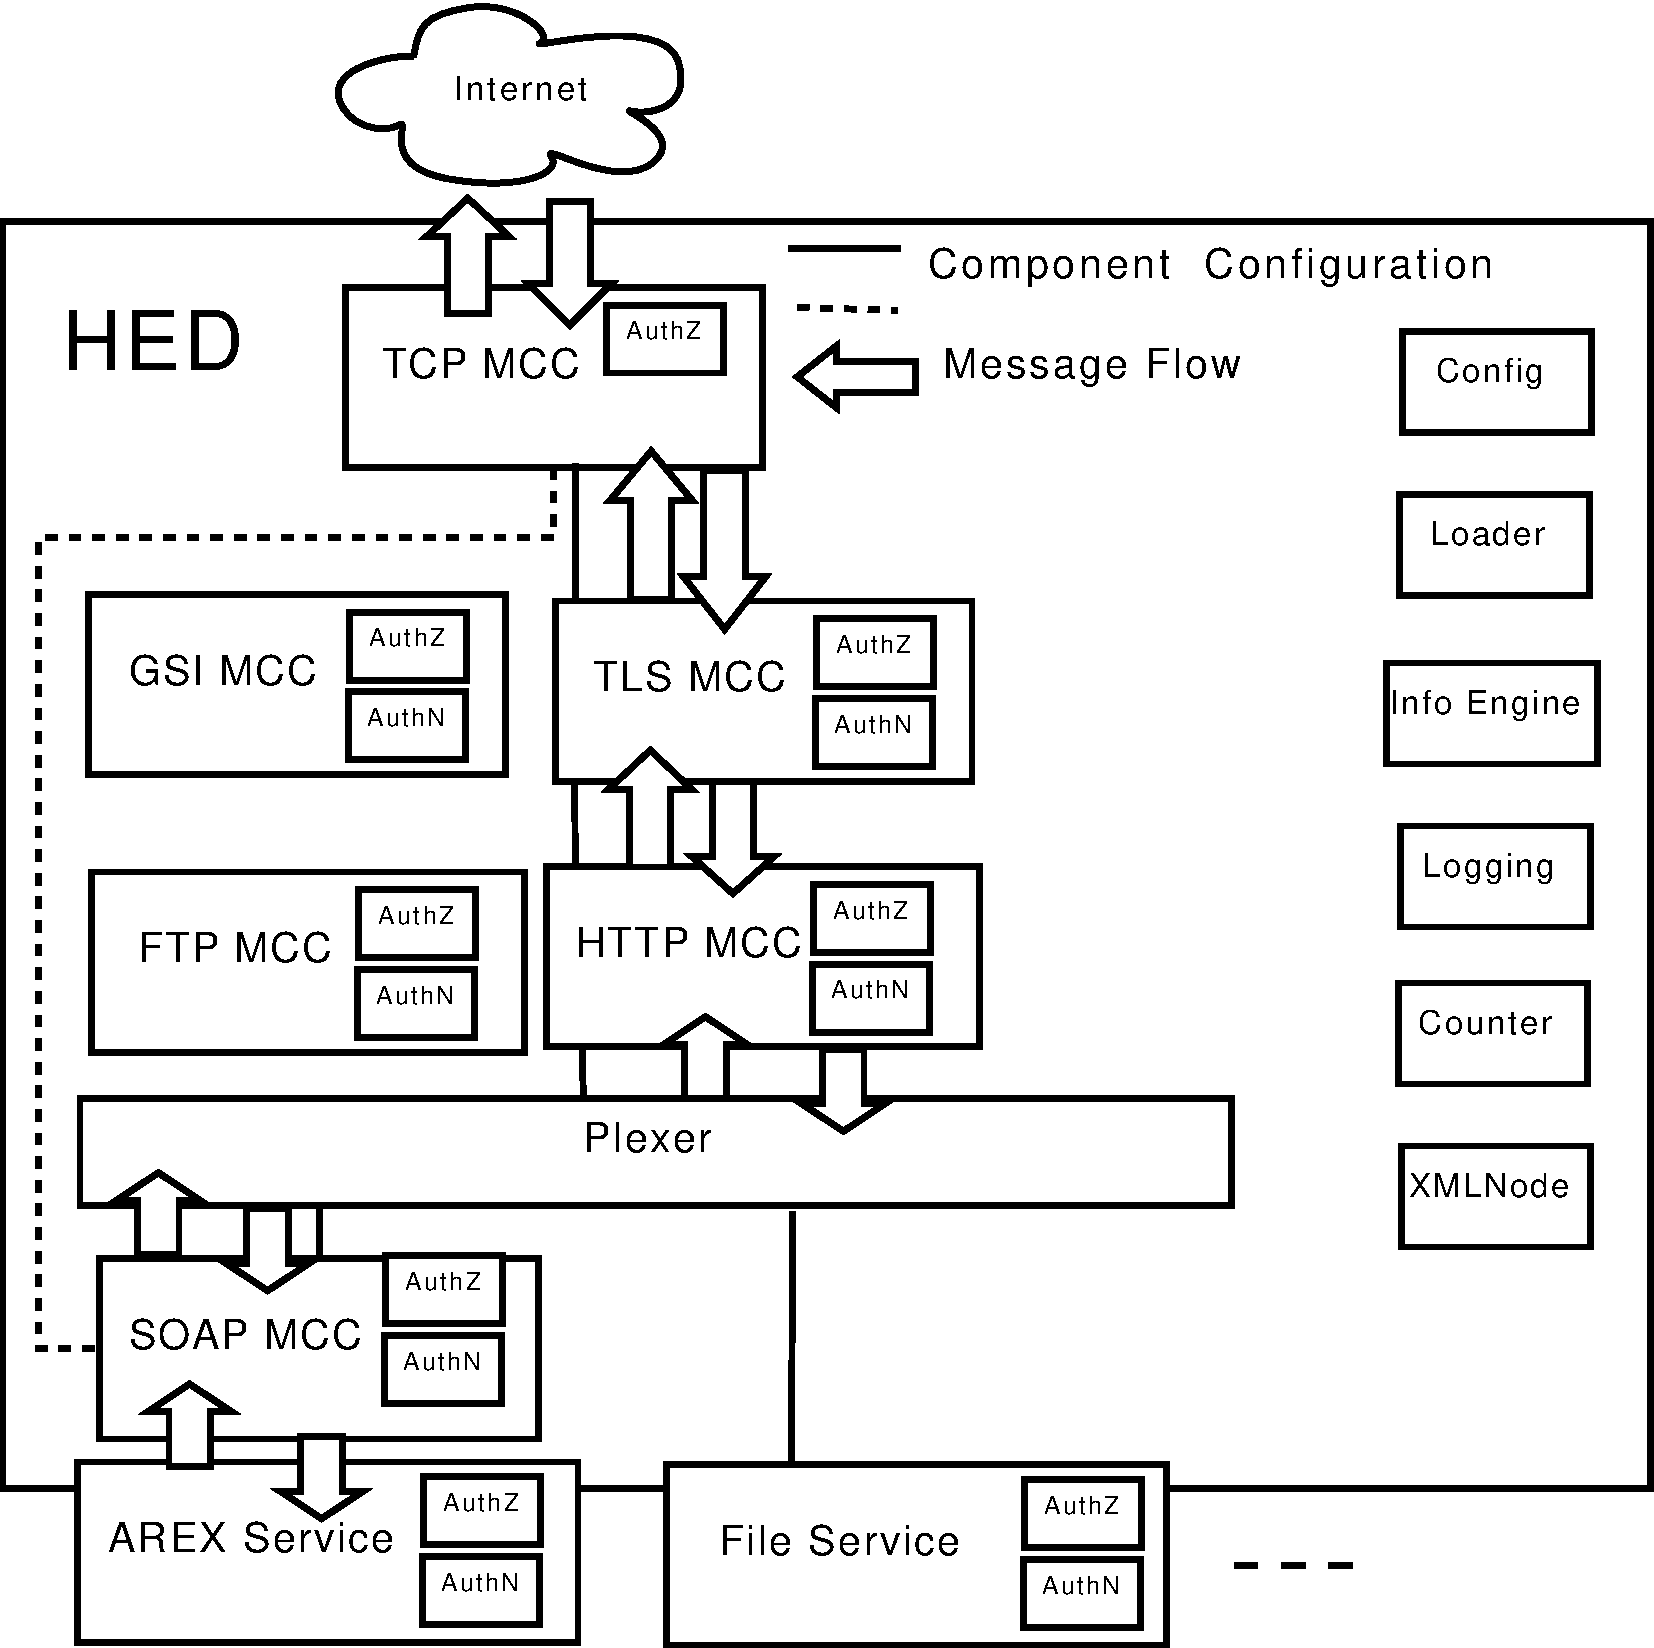
\includegraphics[width=0.9\columnwidth]{HED.pdf}
\caption{The example of Host Environment Daemon deployed with A-REX and File services}
\label{fig:HED}
\end{figure}

HED contains a flexible security framework for implementing and enforcing security 
related functionality, such as authentication and authorization. 
Each security related functionality can be implemented as a pluggable and configurable 
component (plug-ins) called SecHandler. Each MCC or Service is usually configured with 
two queues of SecHandler -- one for the incoming message and one for the outgoing message 
respectively. In Figure \ref{fig:HED}, the ``AuthZ'' and ``AuthN'' sub-modules inside 
MCCs and Services are examples of SecHandler.

%-------------------------------------------------------------------------
\section{Grid authentication using federated identity: Integrating SAML2SSO profile}
\label{sec:intergrationSAML2SSO}
Identity federation is an emerging technology which enables the identity information to be 
trustily transfered across autonomous security domains. By using identity federation, users 
from one domain can access another domain without the need for directly trust relationship 
between users and accessed domain, i.e., users can use accounts from their host domains to 
access external domains, and accessed domain does not need to maintain accounts for those 
external users. Identity federation doesn't enforce specific authentication mechanisms, so 
that various types of authentication can be supported between user and its host domain, and 
user is able to use his frequently used account/credential to accomplish authentication. 
Considering the Grid use cases, we see that utilizing the existing account to access Grid 
without being bothered to applying and manipulating a X.509 credential should be attractive 
for Grid users.

Shibboleth is the one of the several implementations of the identity federation, which is 
based on the OASIS Security Assertion Markup Language (SAML) 2.0 specifications. In terms 
of authentication, the Shibboleth implements SAML2.0 web browser SSO profile, which  defines 
two functional components, an Identity Provider and a Service Provider. The Identity Provider 
(IdP) is responsible for creating, maintaining, and managing user identity, while the Service 
Provider (SP) is responsible for controlling access to services and resources by analyzing 
the SAML assertions produced and issued by the IdP upon request.

In the implementation of ARC middleware, SAML2.0 web browser SSO profile is supported by 
implementing the functionality of service provider and web browser's user agent, and utilizing 
Shibboleth IdP implementation for the functionality of identity provider. The user agent 
functionality is for mimicing the behavior of web browser's user agent for authentication, 
such as the HTTP redirection and the HTTP cookie processing. The implementation of the user 
agent is based on the the HTTPS client interface of ARC, since the client interface of ARC 
can support different protocols which are incarnated by different MCCs.

\begin{figure}
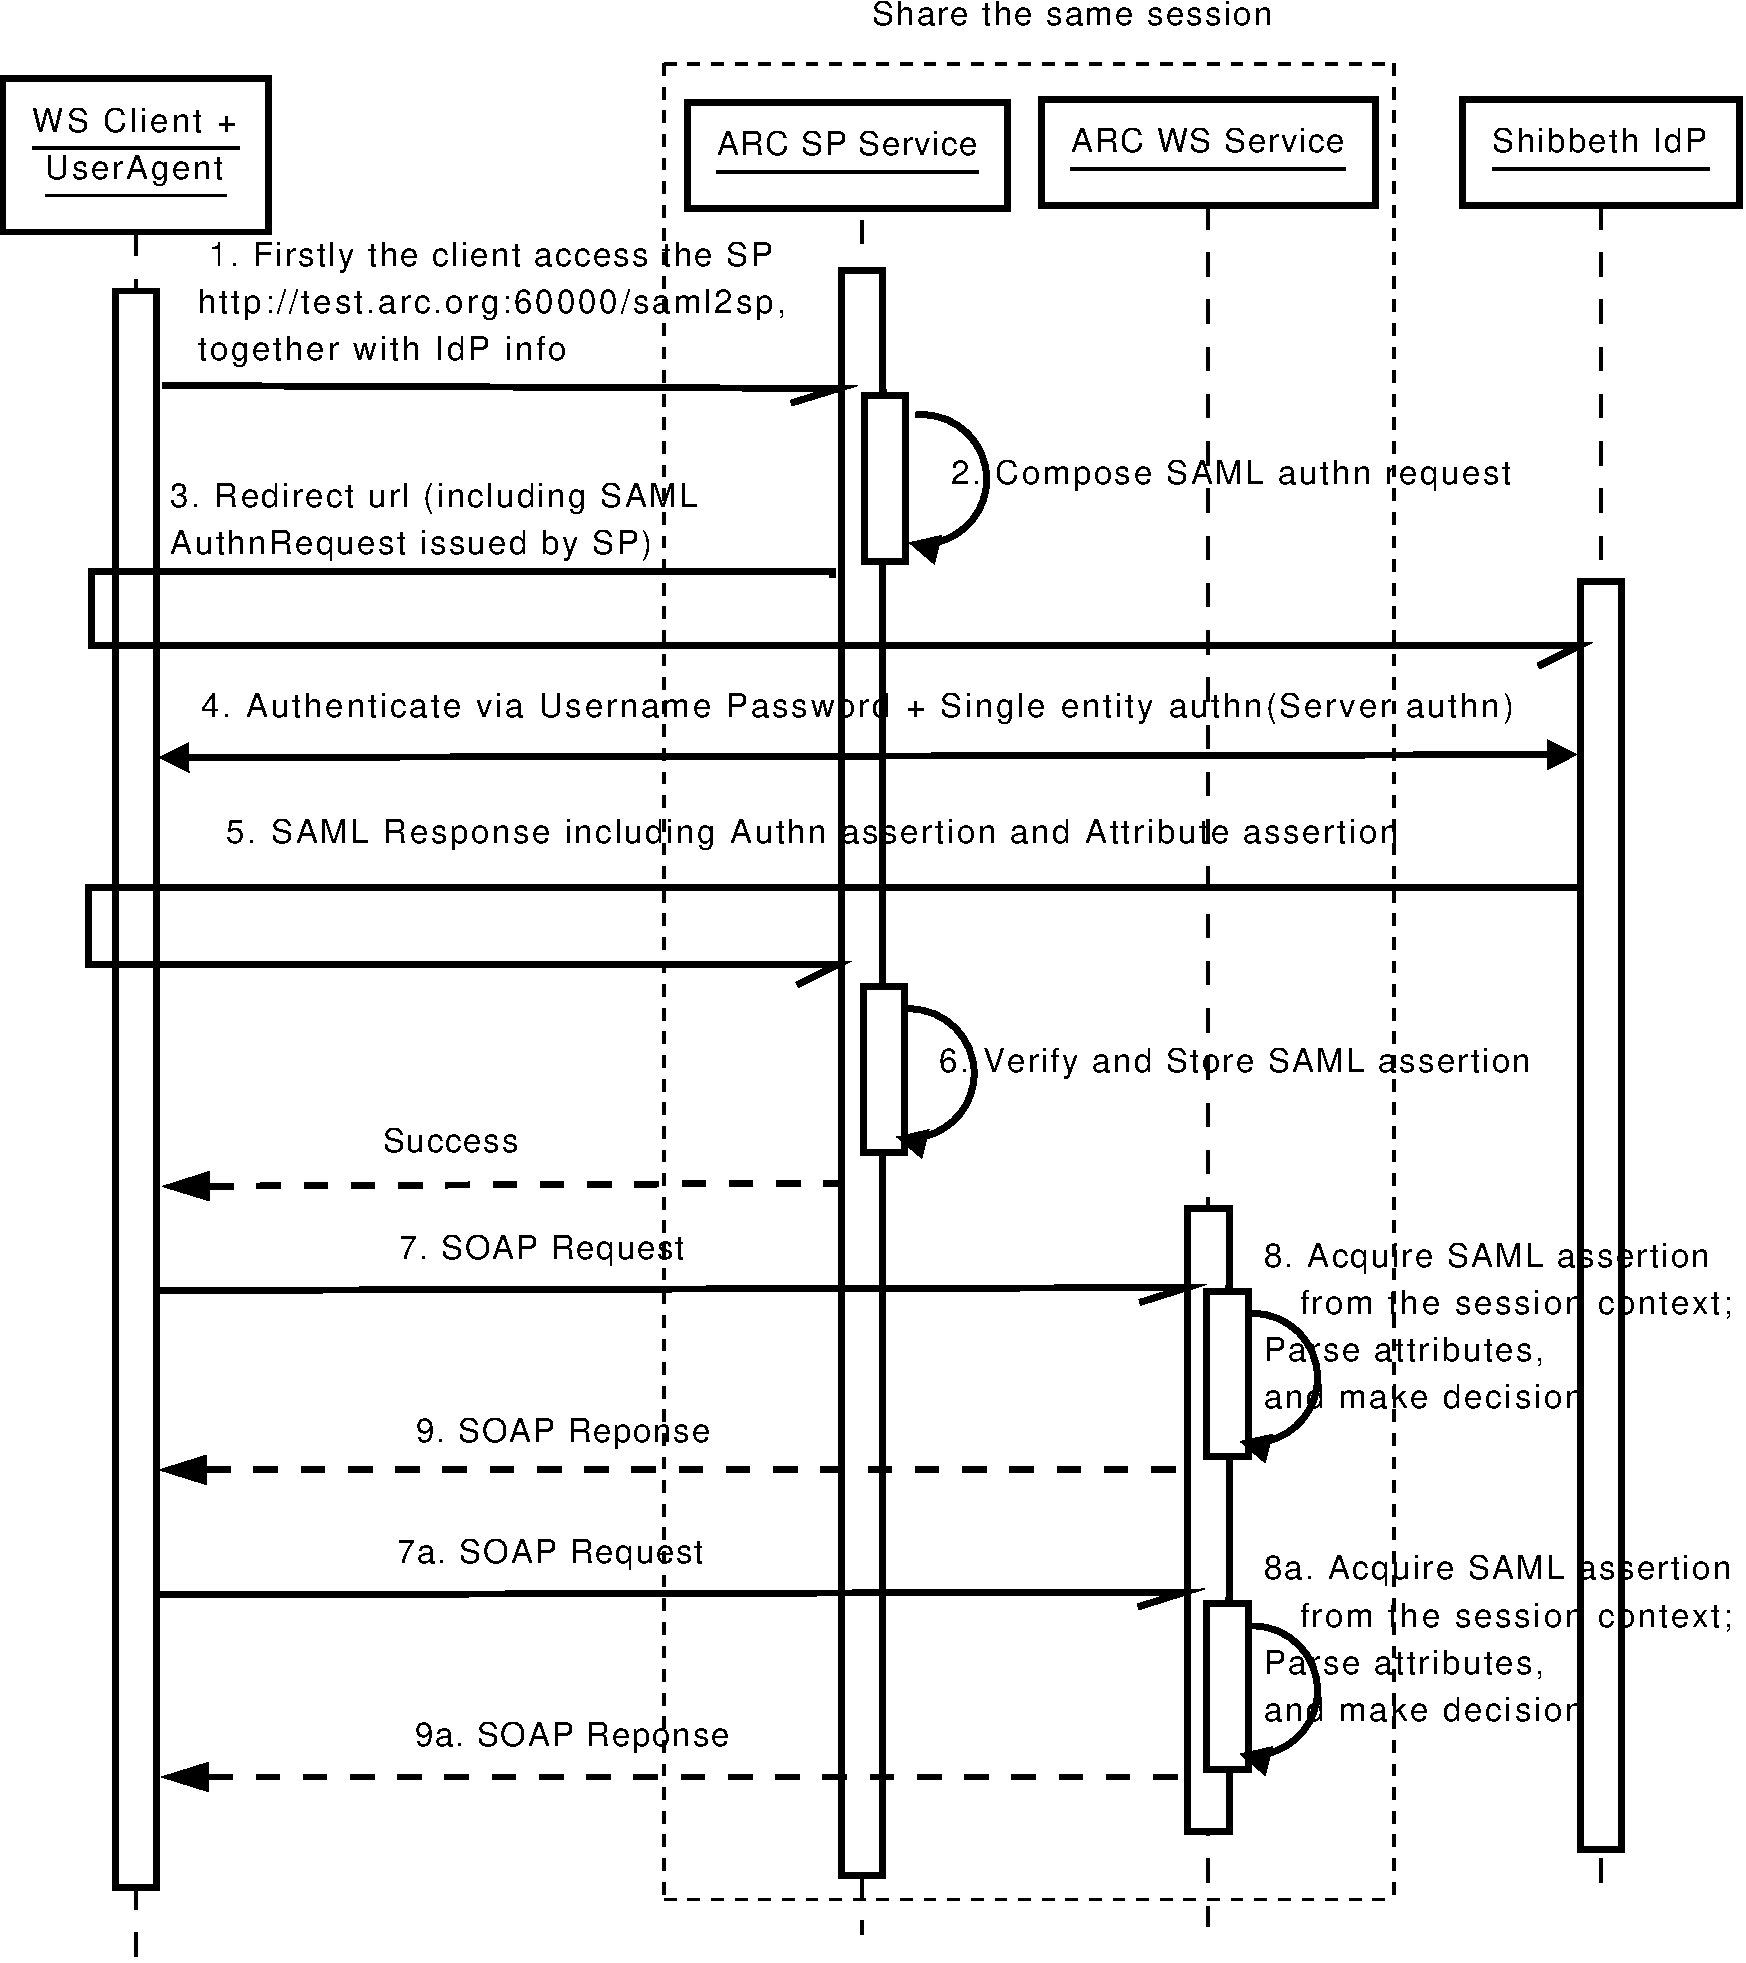
\includegraphics[width=1.0\columnwidth]{SAML2SSO_UML.pdf}
\caption{Sequence diagram of SAML2.0 SSO profile integration in SOAP invocation 
between ARC WS Client and Web Service}
\label{fig:SAML2SSOUML}
\end{figure}

Figure \ref{fig:SAML2SSOUML} shows how is SAML2.0 SSO profile integrated into the SOAP 
invocation between ARC WS Client and Web Service. Step 1 to step 5 in Figure \ref{fig:SAML2SSOUML} 
is similar to those steps depicted in Web Browser SSO profile[ref], with the differences that
we specify the way about how does the service provider determine which identity provider to use (identity
provider discovery), by enabling the client to send the IdP name to service provider; as well 
as specify the way about how does the client/user agent authenticate against service provider, 
by implementing the form-based HTTP authentication which uses username and password for authentication between 
user agent and service provider (rather than X.509 client authentication) and is compatible 
with the Username/Password login handler of Shibboleth IdP.

In step 6, the service provider (SP Service) verifies and checks the SAML response, decrypts and stores 
the SAML assertion into session/connection context. That assertion includes the AuthnStatement and 
AttributeStatement elements. From step 7 to step 9, the WS client launches the SOAP invocation via 
the same connection as the one which is used by user agent to contact SP Service, then Grid/Web Service 
checks the AuthnStatement stored in the session context to see if the AuthnStatement is valid or expired. 
If valid, service handles the SOAP request and returns the SOAP response to the WS client.

Note that in the current implementation the service requires WS client to reuse the same 
TCP connection as the one used by user agent in step 5, in order to guarantee that the validity of 
the SAML2SSO result is applicable to the SOAP invocation process. On the service side, 
the sesion reusing is accomplish by deloying the SP service and other functional Grid/Web Service(s) 
together in the same service container. 

There are a few benifits about integrating SAML2.0 SSO profile for Grid/Web service authentication. 
Firstly, the client certificate authentication can be switched off, so that users do not need 
to apply and maintain a X.509 credential. Secondly, some implementation of identity provider, such as 
Shibboleth IdP, can cache the authentication result through session management once the user
has succeeded to authenticate, and for a short period this authentication result is valid, so that 
the next time the user authenticates against IdP, the user agent can just feed IdP with the last 
successfully authenticated session's identity rather than feed IdP with username and password again. So 
the user (or the client on behalf of that user) can travel across multiple security domains with 
only providing his name and password once, which is also the characteristic of single sign-on.
Lastly, even though there are a few implementations of identity providers, most of them are 
standard-compliant, so the solution implemented in ARC middleware can interoperate with other 
identity provider implementations with minimum change.

%-------------------------------------------------------------------------
\section{Bridging federated identity and X.509 credential}
\label{sec:fedidtoX509}
Many widely used Grid middlewares are based on GSI which requires mutual X.509 authentication. 
Meanwhile, Web Service based Grid applications mostly do require client certificate authentication.  
To bridge the gap beween federated identity and X.509 credential, a short lived credential 
service (SLCS) is implemented through which a user can get a short-lived X.509 certificate only by
providing his username/password and authenticating through the SAML2SSO profile.

Also, in order to provide single sign-on capability for services that act on behalf of user to 
invoke other services, a X.509 credential delegation service is implemented, which is based on 
SOAP communication rather than the proprietary GSI communication implemented in Globus Toolkit.

\subsection{Short-lived credential service}
\label{sec:slcs}
The sequence diagram of SLCS process specializes the diagram shown in Figure \ref{fig:SAML2SSOUML}, 
with the SOAP request including X.509 request and SOAP response including X.509 response. 
In detail, the SLCS client firstly accomplishes the SAML2SSO profile, then sends 
SOAP request to the SLCS service with the X.509 request embedded. The SLCS service makes
access control decision according to the SAML assertion stored in session context, and issues 
a certificate (with 12 hours lifetime) with the SAML attributes as the X.509 certificate 
extension. The SLCS client then gets the SOAP response with the X.509 certificate embedded.

Since the lifetime of the short lived credential has a short lifetime, it is permissible to protect 
the private key by using the local file system permissions instead of encrypting it by 
using a pass-phrase. Therefore, no manual interactivity is required to uncrypted the private
key. Hence single sign-on is provided, since the user only needs to input his password when 
he starts SAML2SSO profile.

How to compose a distinguished name (DN) for the certificate is a critical issue for 
the SLCS service. We pick up the relatively identical information ``eduPersonPrincipalName'' 
(see eduPerson schema~\cite{eduSchemalink}) from SAML attributes that returned from Shibboleth
IdP, and use it to compose the DN. A typical example of the eduPersonPrincipalName 
could be alice@example.org. In such case composed DN is for example\\``/O=knowarc/OU=example.org/CN=alice''.

By using the SLCS service, the user can easily access the Grid services that requires 
X.509 credential on client side, at anywhere, simply by running the SLCS client command 
and providing his username and password.

\subsection{X.509 credential delegation service}
\label{sec:creddeleg}

\begin{figure}
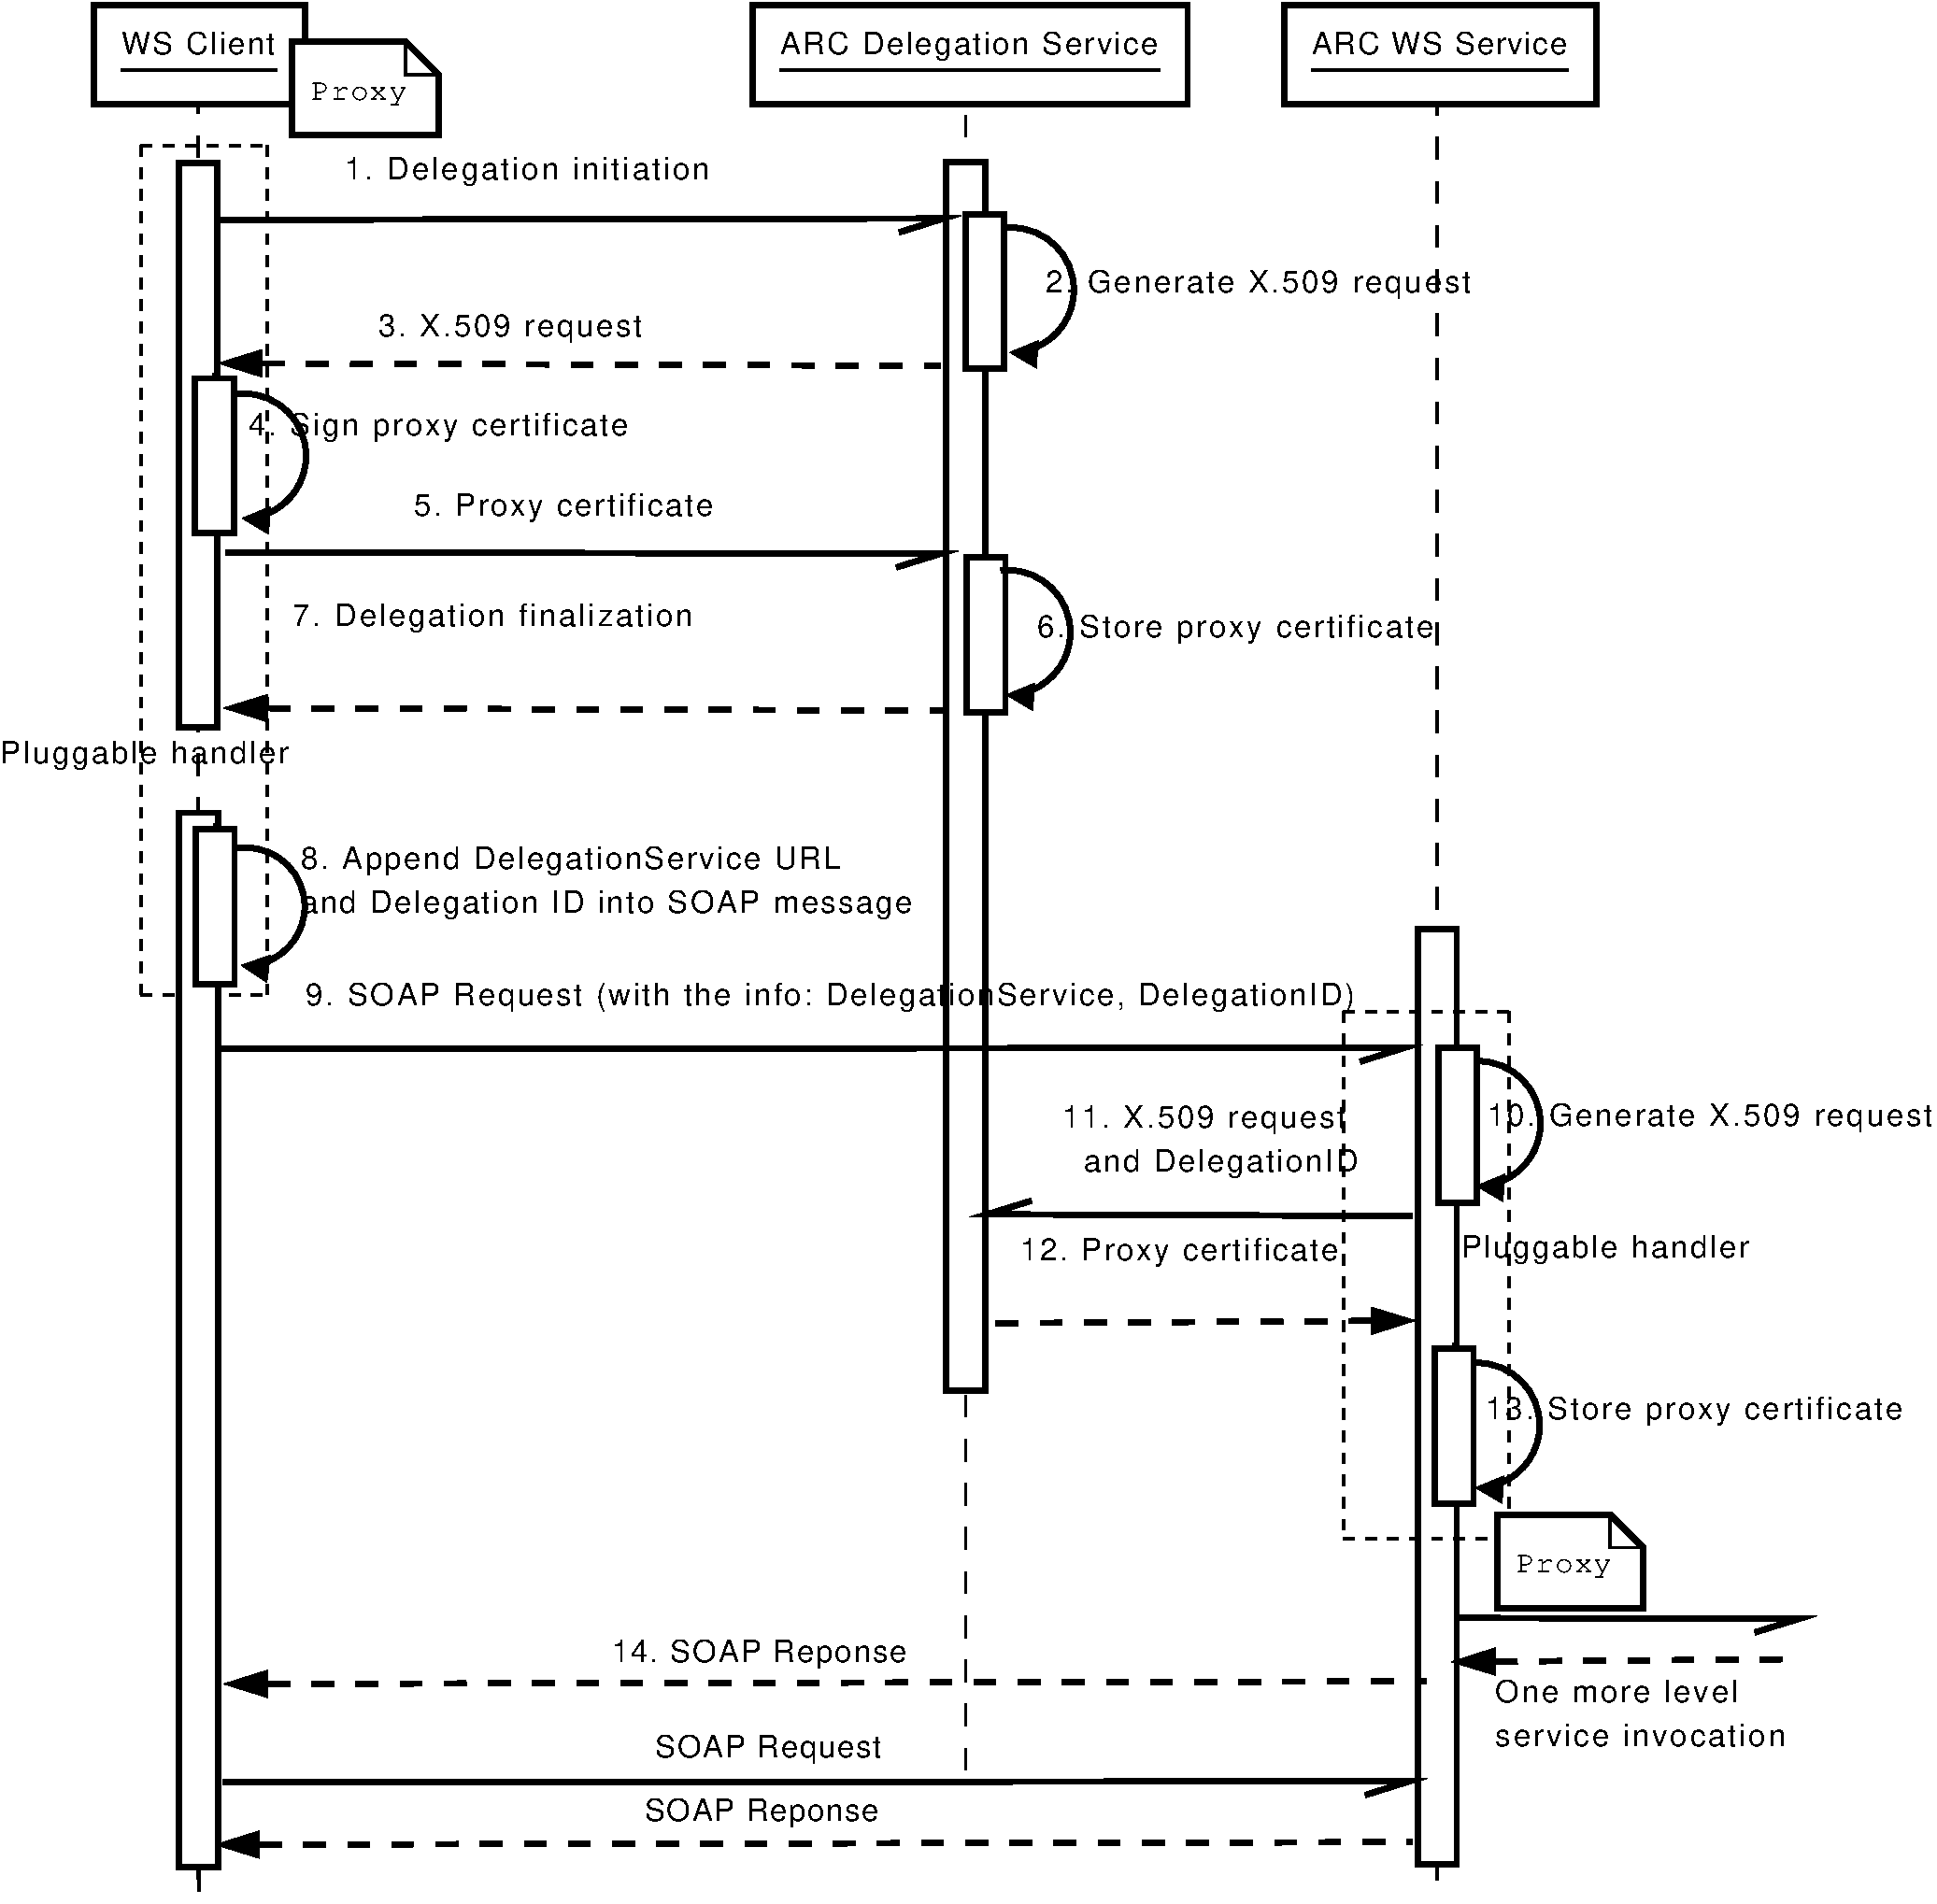
\includegraphics[width=1.0\columnwidth]{Delegation_UML.pdf}
\caption{Sequence diagram of the usage of delegation service}
\label{fig:DelegUML}
\end{figure}

The sequence diagram is shown in Figure \ref{fig:DelegUML}. Firstly, the client needs to delegate
the proxy certificate or short-lived certificate to a delegation service through step 1 to step 7.
Then this client invokes the peer Web Service by appending the delegation information (URL of delegation
service and the delegation ID corresponding to the above delegation) into the SOAP body as out-of-band 
message. The Web Service then sends a X.509 request and the delegation ID to the delegation service 
which is specified by client side, and gets back a delegated certificate which can be composed together
with the private key for a proxy certificate. The Web Service could use this proxy certificate 
to represent the user to invoke another Web Service, which either could cause one more process of 
delegation (step 1 to step 13) if another delegation service is specified, or could directly start
from step 8 if the same delegation service is specified as the one in the former delegation process.

The client only needs to delegate the certificate to delegation service one time per session, it does
not need to do delegation for subsequent SOAP invokations after the first one.

The functionality of both client and service sides are implemented as pluggable handlers which can be 
configured into the client and service configuration, so that the service or client implementation itself
does not need to be changed.

We suppose the short-lived certificate is used by client, so that the SLCS service together with
the delegation service can provide single sign-on from user's federated identity, while keeping the 
interoperability to those Grid/Web services that requires mutual authentication using certificate.

%-------------------------------------------------------------------------
\section{Performace Evaluation}
\label{sec:perfeval}
The following sections evaluate the performance of the HED versus Axis2/C, as 
well as the performance about the SAML2SSO profile, short-lived credential
service, and delegation service.

\subsection{Performance comparison between HED and Axis2/C}
\label{sec:perhedandaxis}
Since the implementation of HED includes an alternative SOAP implementation which is the base of 
the security related web servies described in this paper, it is useful to compare the performance 
of HED and other SOAP implementations. Although there are many SOAP implementations such as 
AxisJava, gSOAP, XSOAP4, etc., the goal of this paper is not about complete comparison between
HED and all the other SOAP implementations, so we use the Axis2/C (v1.5.0) to demostrate the performance
HED.

For the service side, we implement the simple ``echoString'' service in HED, and use the ``echoString''
service in Axis2/C. For client side, we develope a client by using API of ARC, to invoke the ``echoString''
services from Axis2/C and HED. The service invocation is just sending a short string to service, and 
getting back the same string. One test/experiment consists of a set of clients which run simultaneously. 
Each client runs for a fixed period of time, and invokes the service as many times as it can during 
the test period. Multiple clients are launched by creating multiple threads in one test.
Two values are measured: average response time and throughput. Average response time is computed
by counting the average value of the response time for each invocation. Throughput is computed
by counting the number of invocation during each second.

The two ``echoString'' services run in a test machine equipped with 3GHz Intel Pentium dual-core 
CPU and 2GB memory, Red Hat Enterprise Linux 5. The client runs in another machine equipped 
with 1.8GHz Intel Pentium CPU and 2GB memory, Ubuntu 8.10. The Axis2/C service is run using 
the httpd module on Apache Http Server version 2.2.11 instance. We keep all the configurations 
default in Apache Http Server. The client and service are configured with mutual TLS authentication.

\begin{figure}
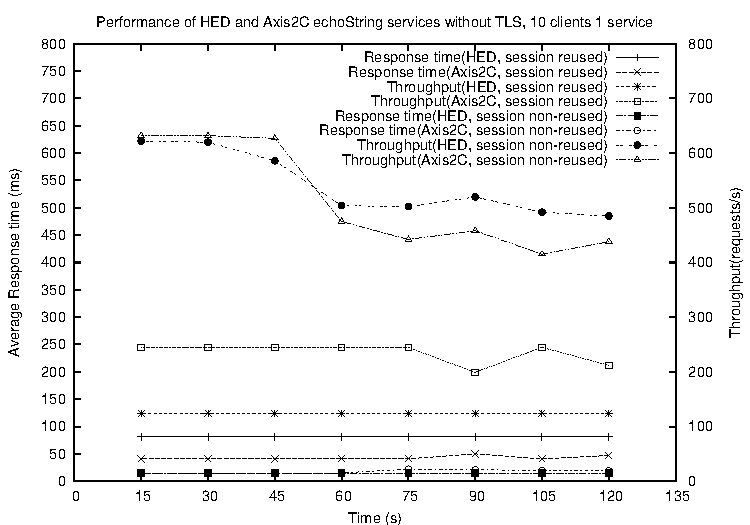
\includegraphics[width=0.9\columnwidth]{HED2Axis_thread10.pdf}
\caption{Performance results for HED and Axis2C: 1 service and 10 clients}
\label{fig:HED2Axis_thread10}
\end{figure}

\begin{figure}
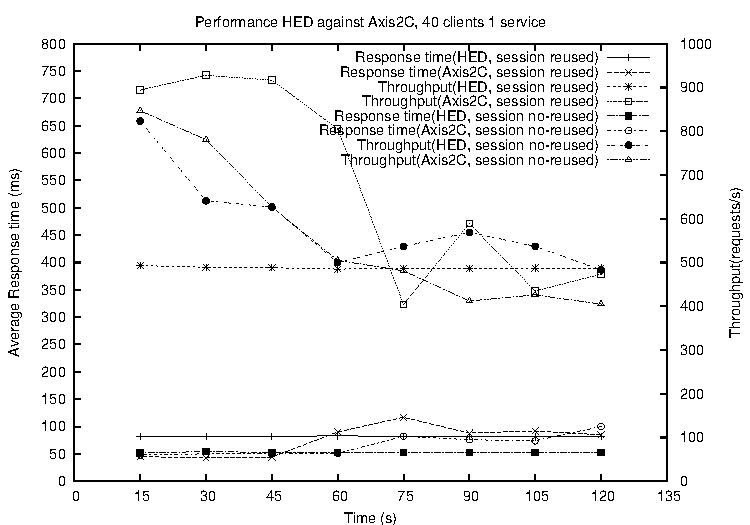
\includegraphics[width=0.9\columnwidth]{HED2Axis_thread40.pdf}
\caption{Performance results for HED and Axis2C: 1 service and 40 clients}
\label{fig:HED2Axis_thread40}
\end{figure}

Figure \ref{fig:HED2Axis_thread10} and Figure \ref{fig:HED2Axis_thread40} are the results of 
performance comparison. 
Two types of experiments are shown: session reused, session non-reused.
``Session reused'' means all of the SOAP invocations on each client share the same session 
(tcp connection); while ``Session non-reused'' means each invocation launches a new session.

For ``Session reused'' experiments, we see that the average response time in HED is about 81ms
which is twice of the value in Axis2/C, and the throughput in HED is about half of the value in Axis2/C, 
when the client number is 10. When the client number is increased to 40, the average response 
time in HED is close to the value in Axis2/C when the duration is more than 60 seconds, and the 
similar result appears for throughput. One obersavation is that, the performance results of HED is 
quite stable, with the average response time almost kept unchanged under different time points, 
as well as under different number of clients, and throughput kept unchanged under different 
time points, while increased linearly with number of clients.

For ``Session non-reused'' experiments, the average response time in HED is almost the same as
the value in Axis2/C, in both cases of client number is 10 (the value is 15ms) and 40 (the value
 is 53ms) correspondingly. On the other hand the throughput in HED is also the same as the value 
in Axis2/C, in both cases of client number is 10 and 40. One interesting obersabation is that the 
throughput is close to a fixed value (around 500 request/s) for both HED and Axis2/C in both 
cases of client number, when the duration value becomes bigger. Also, in case of client number is
40, the throughput from ``Session reused'' experiments also is close to the same fixed value.
We speculate that, with a relatively big value of client number, no matter the session is reused or
not, the throughput is becoming a fixed value which can be explained as the SOAP processing capability
of the SOAP implementation. In this case, we can believe that HED has the similar performance 
capability as Axis2/C. 

\subsection{Performance of the integration SAML2 SSO profile}
\label{sec:perfsaml2sso}
In our next experiment, we evaluate how does the integration of SAML2SSO profile impact on the 
performance of Web Service invocation. We configure a ``echoString'' service together with a SP (
Service Provider) service, and develope a client by using SAML2SSO related API of ARC, to invoke 
the ``echoString'', as well as interact with the IdP (Identity Provider). Services and client run on
the same set of machine as section \ref{sec:perhedandaxis}. Meanwhile, we deploy the Shibboleth IdP 
implementation on a machine equipped with 2.8GHz Intel Pentium CPU and 1GB memory, Red Hat Enterprise 
Linux 5.

\begin{figure}
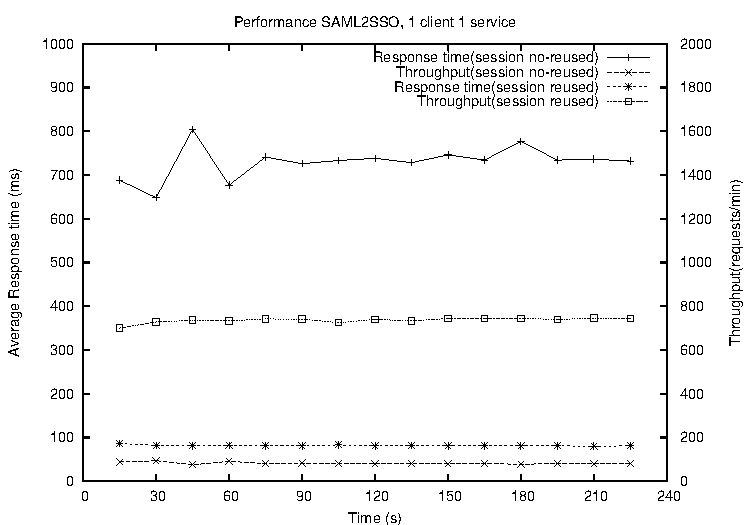
\includegraphics[width=0.9\columnwidth]{SAML2SSO_thread1.pdf}
\caption{Performance results for SAML2SSO profile: 1 service and 1 client}
\label{fig:SAML2SSO_thread1}
\end{figure}

Figure \ref{fig:SAML2SSO_thread1} depicts the average response time and throughputs for one client 
running against the service. Since the success of authentication from IdP can be regarded as 
valid for the whole session between client and service, the client with ``Session reused'' 
need to accomplish the SAML2SSO profile only once for all SOAP invocations on this client, 
while the client with ``Session non-reused'' will need to accomplish this profile once per 
SOAP invocation.

The average response time of ``Session non-reused'' experiments changes little with the execution 
duration, and the value is about 730ms; while the throughput is around 82 requests per minutes.
Considering that the average response time in case of 
``Session non-reused'' and pure SOAP invocation is around 15ms when client number is 10 (see section
\ref{sec:perhedandaxis}), not demostrated in section \ref{sec:perhedandaxis}, the same value applies 
when client number is only 1, therefore we can calculate that the consumption of time for 
SAML2SSO profile is about 98\% of the whole SOAP invocation with SAML2SSO profile integrated.
Deeper investigation about recording the time of each step of SAML2SSO profile supports the above
obersavation. In order to improve the performance of SAML2SSO profile, optimizing the process between
client and IdP is the correct direction, and probably one of the easiest way is to enhance the 
hardware configuration.

One the other hand, the average response time of ``Session reused'' experiments is about 82 ms,
which is almost as short as the value in the pure SOAP invocation experiment in \ref{sec:perhedandaxis}.
The result is resonable because the time consumption caused by only once of SAML2SSO execution on one 
client is relatively small comparing with the time consumption caused by the following hundreds 
of pure SOAP invocations.

\begin{figure}
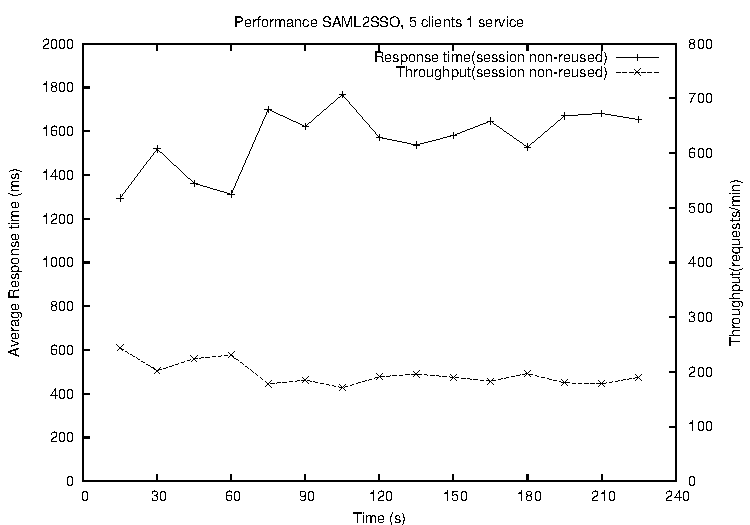
\includegraphics[width=0.9\columnwidth]{SAML2SSO_thread5.pdf}
\caption{Performance results for SAML2SSO profile: 1 service and 5 clients}
\label{fig:SAML2SSO_thread5}
\end{figure}

\begin{figure}
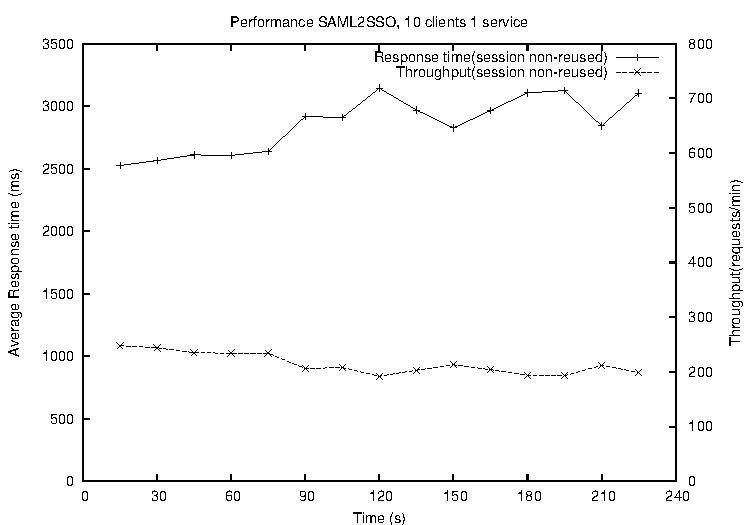
\includegraphics[width=0.9\columnwidth]{SAML2SSO_thread10.pdf}
\caption{Performance results for SAML2SSO profile: 1 service and 10 clients}
\label{fig:SAML2SSO_thread10}
\end{figure}

Figure \ref{fig:SAML2SSO_thread5} and Figure \ref{fig:SAML2SSO_thread10} depicts the average 
response time and throughputs for 5 and 10 clients running against one service simultaneously,
with the session not being reused. The throughput seems to change little with the number of 
clients increased from five to ten, with the value being abroud 200 requests per minutes;
while the average response time doubles, with the value increasing from 1.6s to 3.1s. We conclude
that in order to get acceptable response time, there should be at least less than five concurrent
clients if they need to continuously participate one SAML2SSO profile. 

However for some typical grid application scenarios, normally the client does not need 
to continuously accomplish SAML2SSO profile. For instance, a user could submit a job 
which needs a period of time (normally this period is much longer than a few seconds)
to execute, which launches an execution of SAML2SSO profile; 
afterwards, this user could query the information as well as the result about this job, which 
launches another execution of SAML2SSO profile. On the other hand, statistically, users will most
probably not access grid system in a concurrent way, rather a random way. Therefore, if we 
suppose a user could access grid once per minute, in our test environment, we can claim that 
around 200 clients randomly can be supported with acceptable performance.


\subsection{Performance of SLCS service}
\label{sec:perfslcsserv}

\begin{figure}
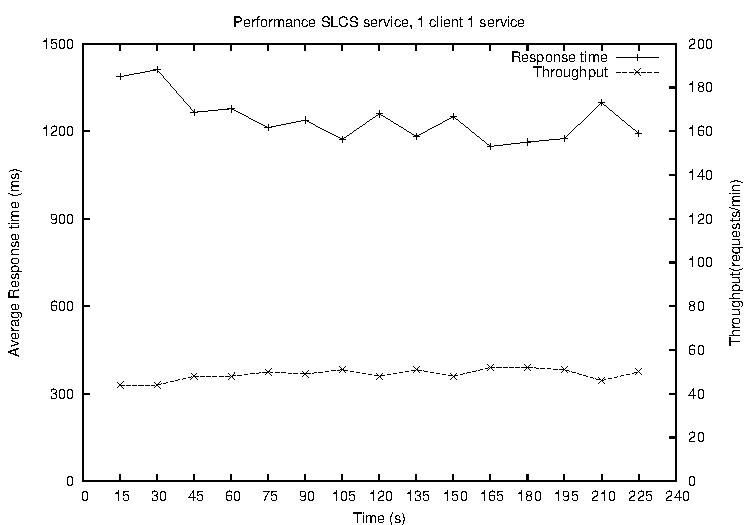
\includegraphics[width=0.9\columnwidth]{SLCS.pdf}
\caption{Performance results for SLCS service: 1 service and 1 client}
\label{fig:SLCS}
\end{figure}

Figure \ref{fig:SLCS} is the performance about the SLCS service. Since the SLCS is based on the SAML2SSO
profile, the reponse time should be the accumulation of time consumption about the SAML2SSO processing 
and the SLCS processing. In this experiment, SLCS service and client run on the same set of machine 
as section \ref{sec:perhedandaxis}. This figure shows that the average response time changes little with
the execution time with the value being around 1.3s which is nearly double as the value (730ms) of one client 
experiment about ``echoString'' service invocation with SAML2SSO integrated. Not demostrated in 
Figure \ref{fig:SLCS}, the more consumption of time is caused by the creating of X.509 request on the
 client side, which takes about roughly 310ms in average, as well as by the signing of X.509 certificate 
on the SLCS service side, which takes roughly 33ms in average, together with the time consumption for 
communication.

Even though the average response time of SLCS service is not very short, considering the short-lived 
credential has a relatively long lifetime (12 hours by default) and therefore client only needs to invoke
SLCS service once per 12 hours, the performance is completely acceptable. Also considering the time 
consumption for the creation of X.509 request (1024-bit RSA key pair generation) is on the client side,
we speculate the SLCS service side will not be affected much by the time-consuming key pair generation, and
therefore its performance resemble the performance of SAML2SSO profile in section \ref{sec:perfsaml2sso}.

\subsection{Performance of delegation service}
\label{sec:perfdelegserv}

In the last experiment, we evaluate how does the usage of delegation service impact on the 
performance of Web Service invocation. We deployed a ``echoString'' service plugged with delegation
security handler on a machine equipped with 2.80GHz Intel Pentium CPU and 1GB memory, Red Hat 
Enterprise Linux 5, and also configure a client together with delegation security handler plugged 
on a machine equipped with 1.8GHz Intel Pentium CPU and 2GB memory, Ubuntu 8.10. Aside from 
``echoString'' service and client, a delegation service is deployed on a machine equipped with 
3GHz Intel Pentium dual-core CPU and 2GB memory, Red Hat Enterprise Linux 5.

\begin{figure}
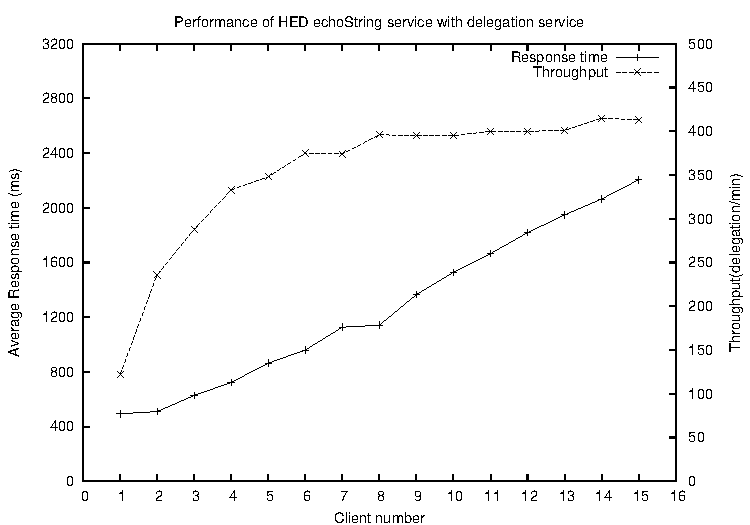
\includegraphics[width=0.9\columnwidth]{Delegation_thread_to_perf.pdf}
\caption{Performance results of delegation service: from 1 client to 15 clients}
\label{fig:Deleg}
\end{figure}

Initial experiments which are not demonstrated in this paper show that both the response time and
throughput almost do not change with the time. Therefore, we measure the performance as the function 
of the client numbers from 1 to 15. Figure \ref{fig:Deleg} is performance results. We see that 
the response time increases in a linear manner against client numbers; and the throughput gradually 
increases, and stops increasing and almost keeps unchanged when the client number is bigger than eight.
We conclude that if the client number is bigger than eight, in our test environment, there is no 
throughput benefit can be achieved by adding clients.


%-------------------------------------------------------------------------
\section{Related Work}
\label{sec:relatedwork}
There are other researches that utilize Shibboleth for protecting usage of Grid resources. 
The work in ~\cite{J.Watt06} uses Shibboleth to protect a GridSphere portal and then 
indirectly protect Grid services which are deployed in this GridSphere protal. Another 
work in ~\cite{R.O.Sinnott06} also uses Shibboleth to protect Grid portal, moreover, it 
maintains a few common used server certificates which can then be used to access Grid 
resources after users have successfully authenticated themselves at Grid protal through
Shibboleth. Unlike these two solutions that use Shibboleth to protect Grid portal, the solution
in this paper uses Shibboleth or similar standards-based identity federation to directly protect 
Grid resource/services, which provide possibility for those Grid applications that are directly
based on Grid interface (e.g., applications that invokes SOAP operations of remote Grid services),
to benefit from identity federation.

GridShib~\cite{T.Scavo07,VWelch05} provides one solution that users can use X.509 
certificate to authenticate to Shibbolth IdP, get back SAML assertion and embed it in 
the proxy certificate. The Grid service will then use this SAML assertion for access control.
Unlike the work described in this paper, GridShib still requires users to possess a X.509 
credential, rather than username/password. GridShib also provides another 
solution~\cite{TBarton06} in which a credential service (MyProxy server) is deployed together
with Shibboleth IdP for acting as an online-CA, authenticating the user through username/password
rather than X.509 certificate, and issuing short-lived X.509 credential. The second solution
is similar to the short-lived credential service in our solution, while our solution
also provides the option for users directly authenticating to Grid services via SAML2.0 SSO 
profile using their username/password.

Another short-lived credential service is also provided by ~\cite{switchslcslink}. 
The advantage of our work comparing to the work in ~\cite{switchslcslink} is that 
our SLCS service is based on Web Services standard, so that it is easier to achieve 
interoperability.

In the aspect of credential delegation, apart from the credential delegation mechanism of 
GSI~\cite{IFoster98,VWelch04}, several authors~\cite{MAhsant04} propose a delegation protocol 
based on the WS-Trust~\cite{WSTrustlink} to provide a standard and interoperable protocol 
for the delegation in Grids. WS-Trust will also be adopted by the ARC middleware to express the 
specifications required to define delegation protocol in a standard way. Gridsite project also
implements a X.509 credential delegation solution~\cite{GridSitelink} based on the Web 
Service, with which ARC delegation client can be easily made interoperate.

%-------------------------------------------------------------------------
\section{Conclusion And Future Work}
\label{sec:conclusion}
In this paper we propose a Grid single sign-on framework that can utilize users' 
federated identity instead of X.509 mutual authentication for authentication, which
we believe can make further uptake of Grid resources as well as Grid middleware by 
wider scale of users.

We implement the SAML2 SSO profile in the ARC Grid middleware, so that the Grid applications
that developed by using the application interface provided by this middleware can easily 
be switched to benefit from federated identity based authentication. 
The performance evaluation shows even though the introducing of SAML2 SSO profile causes 
much performance downgrade, this downgrade can be avoided by reusing the authentication 
result for multiple SOAP invocations.
Meanwhile, in order to be compatible with those Grid applications that require X.509 
certificate on the client side, we also implement one Web Service which can be used for 
obtaining an X.509 credential based on federated identity, and the other Web Service 
which can be used for delegating X.509 credential. We believe that the evaluated 
performance is enough for creating X.509 certificate and proxy certificate, considering that 
the certificates should have a relaively much longer lifetime comparing to the response time of 
these two services.
 
Although only authentication issue has been discussed in this paper, we know single
sign-in should also include the authorization issue. The SAML assertion which includes
users' attributes can be used on the serrvice side to achiece attribute-based authorization.
Therefore providing plugin on the service side to enforce access control using SAML attribute
is considered one part of the future work.

SimpleSAMLphp~\cite{simplesamllink} provides another implementation of SAML2 SSO profile, and it 
has been widely deployed around nordic countries for identity federation. Hence integrating
ARC based Grid applications with simpleSAMLphp is considered as another of future work.



% An example of a floating figure using the graphicx package.
% Note that \label must occur AFTER (or within) \caption.
% For figures, \caption should occur after the \includegraphics.
% Note that IEEEtran v1.7 and later has special internal code that
% is designed to preserve the operation of \label within \caption
% even when the captionsoff option is in effect. However, because
% of issues like this, it may be the safest practice to put all your
% \label just after \caption rather than within \caption{}.
%
% Reminder: the "draftcls" or "draftclsnofoot", not "draft", class
% option should be used if it is desired that the figures are to be
% displayed while in draft mode.
%
%\begin{figure}[!t]
%\centering
%\includegraphics[width=2.5in]{myfigure}
% where an .eps filename suffix will be assumed under latex, 
% and a .pdf suffix will be assumed for pdflatex; or what has been declared
% via \DeclareGraphicsExtensions.
%\caption{Simulation Results}
%\label{fig_sim}
%\end{figure}

% Note that IEEE typically puts floats only at the top, even when this
% results in a large percentage of a column being occupied by floats.


% An example of a double column floating figure using two subfigures.
% (The subfig.sty package must be loaded for this to work.)
% The subfigure \label commands are set within each subfloat command, the
% \label for the overall figure must come after \caption.
% \hfil must be used as a separator to get equal spacing.
% The subfigure.sty package works much the same way, except \subfigure is
% used instead of \subfloat.
%
%\begin{figure*}[!t]
%\centerline{\subfloat[Case I]\includegraphics[width=2.5in]{subfigcase1}%
%\label{fig_first_case}}
%\hfil
%\subfloat[Case II]{\includegraphics[width=2.5in]{subfigcase2}%
%\label{fig_second_case}}}
%\caption{Simulation results}
%\label{fig_sim}
%\end{figure*}
%
% Note that often IEEE papers with subfigures do not employ subfigure
% captions (using the optional argument to \subfloat), but instead will
% reference/describe all of them (a), (b), etc., within the main caption.


% An example of a floating table. Note that, for IEEE style tables, the 
% \caption command should come BEFORE the table. Table text will default to
% \footnotesize as IEEE normally uses this smaller font for tables.
% The \label must come after \caption as always.
%
%\begin{table}[!t]
%% increase table row spacing, adjust to taste
%\renewcommand{\arraystretch}{1.3}
% if using array.sty, it might be a good idea to tweak the value of
% \extrarowheight as needed to properly center the text within the cells
%\caption{An Example of a Table}
%\label{table_example}
%\centering
%% Some packages, such as MDW tools, offer better commands for making tables
%% than the plain LaTeX2e tabular which is used here.
%\begin{tabular}{|c||c|}
%\hline
%One & Two\\
%\hline
%Three & Four\\
%\hline
%\end{tabular}
%\end{table}


\section*{Acknowledgment}


The authors would like to thank...


% trigger a \newpage just before the given reference
% number - used to balance the columns on the last page
% adjust value as needed - may need to be readjusted if
% the document is modified later
%\IEEEtriggeratref{8}
% The "triggered" command can be changed if desired:
%\IEEEtriggercmd{\enlargethispage{-5in}}

% references section


%\bibliographystyle{IEEEtran}

\begin{thebibliography}{1}

\bibitem{IFoster98}
I. Foster, C. Kesselman, G. Tsudik, and S. Tuecke, A Security Architecture for 
Computational Grids, ACM Conference on Computers and Security, 1998, 83-91.

\bibitem{AlfieriR05}
R. Alfieri, R. Cecchini, V. Ciaschini, L. dell’Agnello, A. Frohner, K. Lorentey, 
and F. Spataro. From gridmap-file to voms: managing authorization in a Grid environment. 
Future Generation Comp. Syst., 21(4), 549-558 (2005)

\bibitem{RFC3821link}
RFC 3821- An Internet Attribute Certificate Profile for Authorization. http://www.faqs.org/rfcs/rfc3281.html

\bibitem{GTlink}
Globus Toolkit. http://www.globus.org/toolkit/

\bibitem{gLitelink}
gLite: lightweight middleware for Grid computing. http://glite.web.cern.ch

\bibitem{ARClink}
Advanced Resource Connector. http://www.nordugrid.org/middleware/

\bibitem{WSSeclink}
OASIS Web Services Security. www.oasis-open.org/committees/wss/

\bibitem{SAMLlink}
OASIS Security Assertion Markup Languages (SAML). www.oasis-open.org/committees/security/

\bibitem{MEllert07}
M. Ellert et al. Advanced resource connector middleware for lightweight computational 
grids, Future Generation computer systems, 23(2), 219-240 (2007)

\bibitem{KnowARClink}
KnowARC project.  https://www.knowarc.eu/

\bibitem{KnowARCDesignlink}
Design document of new version ARC. https://www.knowarc.eu/documents/Knowarc\_D1.1-1\_07.pdf

\bibitem{WSElink}
Web Services Enhancements 2.0 Service Pack 2. http://msdn.microsoft.com/en-us/library/

\bibitem{A.Shoshan03}
A. Shoshani, A. Sim, and J. Gu, Storage Resource Managers: Essential Components for the Grid, 
Grid Resource Management: State of the Art and Future Trends, Kluwer Publishing, 2003.

\bibitem{Shiblink}
The Shibboleth Project. http://shibboleth.internet2.edu/

\bibitem{eduSchemalink}
eduPerson and eduOrg Object shema. http://middleware.internet2.edu/eduperson/

\bibitem{R.O.Sinnott06}
R.O. Sinnott, J. Jiang, J. Watt, and O. Ajayi. Shibboleth-based access to and 
usage of grid resources. Proceeding of 7th IEEE/ACM International Conference on 
Grid Computing, September 2006, Barcelona.

\bibitem{J.Watt06}
J. Watt, O. Ajayi, J. Jiang, J. Koetsier, R.O. Sinnott. A Shibboleth-Protected 
Privilege Management Infrastructure for e-Science Education. in proceeding of Sixth 
IEEE International Symposium on Cluster Computing and the Grid (CCGRID'06), May 2006,
Singapore.

\bibitem{T.Scavo07}
T. Scavo and V. Welch. A Grid Authorization Model for Science Gateways. International 
Workshop on Grid Computing Environments, 2007.

\bibitem{VWelch05}
V. Welch, T. Barton, K. Keahey and F. Siebenlist. Attributes, Anonymity, and 
Access: Shibboleth and Globus Integration to Facilitate Grid Collaboration. in 
proceeding of 4th Annual PKI R\&D Workshop, 2005.

\bibitem{TBarton06}
T. Barton et al. Identity Federation and Attribute-based Authorization 
through the Globus Toolkit, Shibboleth, Gridshib, and MyProxy. in proceeding 
of 5th Annual PKI R\&D Workshop, 2006.

\bibitem{switchslcslink}
SWITCH Short Lived Credential Service. http://www.switch.ch/Grid/slcs/

\bibitem{VWelch04}
V. Welch et al. X.509 proxy certificate for dynamic delegation. in proceeding 
of the 3rd Annual KI R\&D Workshop, 2004.

\bibitem{MAhsant04}
M. Ahsant, J. Basney, and O. Mulmo. Grid Delegation Protocol. UK Workshop on 
Grid Security Experiences, Oxford. 2004.

\bibitem{WSTrustlink}
OASIS WS-Trust specification. http://docs.oasis-open.org/ws-sx/ws-trust/200512

\bibitem{GridSitelink}
Gridsite delegation service. http://www.gridsite.org/wiki/Delegation\_protocol

\bibitem{simplesamllink}
http://rnd.feide.no/simplesamlphp

\end{thebibliography}




\end{document}


